\documentclass{article}
\usepackage[utf8]{inputenc}
\usepackage{geometry}
\geometry{margin=1in}
\usepackage{amsmath}
\usepackage{amssymb}
\usepackage[ruled,vlined, linesnumbered]{algorithm2e}
\usepackage[english]{babel}
\usepackage[nottoc]{tocbibind}
\usepackage{color}
\usepackage{natbib}
\usepackage{graphicx}
\usepackage{float}
\newtheorem{theorem}{Theorem}[section]
\bibliographystyle{abbrvnat}
% Custom commands / shortcuts
\providecommand{\sign}{\textrm{sign}}
\providecommand{\note}[1]{\textcolor{red}{#1}}
\providecommand{\lam}{\lambda}

\title{Adaptive Safe Strong Screening for Efficient Lasso-Type
Problems Optimization over the Solution Path}
\author{Chuyi Wang\\Department of Statistics and Actuarial Sciences\\University of Iowa
  \and
  Patrick Breheny\\Department of Biostatistics\\University of Iowa}
\date{}

\begin{document}

\maketitle

\section{Introduction}

The lasso (least absolute shrinkage and selection operator) model\citep{tibshirani1996regression}, is a popular model in statistics and machine learning, especially in high-dimensional problems. The model can be defined as the following modification of the least squares optimization problem:
\begin{equation}
    \hat{\beta}(\lambda)=\underset{\beta\in \mathbb{R}^p}{\mathrm{argmin}}\frac{1}{2n}||y-X\beta||_2^2+\lambda||\beta||_1,
\end{equation}
where $y$ is the $n\times 1$ response vector correspond to $n$ observations, $X=(x_1,x_2,...,x_p)$ is the $n\times p$ feature matrix correspond to $p$ features, $\beta\in \mathbb{R}^p$ is the $p\times 1$ coefficient vector and $\lambda$ is the regularization tuning parameter. $||\cdot||_2$ denotes the $l_2$ (Euclidean) norm and $||\cdot||_1$ denotes the $l_1$ norm. 

The lasso model has several attractive properties compared to least squares regression, including increased stability of estimation, increased prediction accuracy, and automatic variable selection arising from the fact that it yields sparse estimates of $\beta$.  As a result, it is widely applied in different fields, such as gene expression data analysis, image recognition and text mining, and has been extended in several ways, such as group lasso\citep{yuan2006model}, elastic net\citep{zou2005regularization} and sparse generalized linear models. Because of its wide popularity, solving the lasso model efficiently is an important topic in statistics and machine learning.

Because the optimal value of $\lambda$ is not known in advance, typical practice is to solve for $\beta$ along a sequence of values of the tuning parameter $\lambda$, known as the solution path.  Pathwise algorithms can be efficiently implemented by using the solution at a previous $\lambda$ value as a ``warm start'' for the next value of $\lambda$.  In particular, the pathwise coordinate descent algorithm\citep{friedman2007pathwise}, which optimizes $\beta(\lambda)$ one element at a time with the remaining coordinates held fixed, has been shown to outperform other lasso algorithms such as LARS (least angle regression)\citep{efron2004least}, especially in high dimensional settings where $p$ is large. In sparse settings, it scales up very well with a computational cost of approximately $O(np)$. 

However, modern data collection and storage techniques allow researchers to measure an increasingly large number of features, which introduce additional computational challenges. In particular, it may not be possible to store the feature matrix, which can require many GBs of memory to store, in memory. One can resolve this problem by using a memory mapping package such as \textbf{bigmemory}, which allows us to store the feature matrix on disk and read it portions of it as needed; however, this results in frequent reading from disk, which is extremely slow compared to other parts of the algorithm and becomes a bottleneck with respect to the computational burden of fitting lasso models on very large data sets.

One promising technique to address this challenge is feature screening. The lasso model solution is sparse in the sense that most coefficients will be exactly zero; for these ``inactive'' coefficients we do not need their associated features.  In theory, if we knew which coefficients were nonzero at each value of $\lambda$, we could read into memory only those features and leave the remaining features on disk. In reality, we cannot know this prior to fitting the model -- however, through the clever use of feature screening rules, we can greatly reduce the number of times inactive features are read into memory, thereby minimizing the computational burden.  In what follows, we refer to features left on disk as ``discarded'' features, although it is worth clarifying that this is not a permanent decision and a decision is made for each $\lambda$ values: for example, a feature can be discarded at one value of $\lambda$ but included in the list of potentially active features at other values of $\lambda$.

There are two important categories of features screening rules: ``strong'' rules\citep{tibshirani2011regression}\citep{qian2019fast}, which occasionally incorrectly discard some active features, and ``safe'' rules\citep{ghaoui2010safe,wang2013lasso,xiang2012fast, xiang2011learning}, which are guaranteed never to do so.  As one might expect, strong rules tend to be easier to calculate; however, because mistakes are possible, one must add a post-convergence check to ensure that no features were incorrectly discarded. This check is not necessary with safe rules. However, safe rules are considerably less powerful at discarding features than strong rules. More recently, hybrid approaches \citep{zeng2017efficient} combining the two types of rules have been shown to be more efficient than either type of rule alone.

Previous safe screening rules can also be divided into two categories, sequential rules and one-step rules, by how the screening is carried out along the path of $\lambda$ values. Sequential rules do heavy computation for each $\lambda$ values using solution from its previous $\lambda$ value, so they are slower but relatively powerful at each $\lambda$ values. One-step rules only require heavy computation at the beginning and thus are faster but they cannot remain powerful along the path for long. 

In this paper, we proposed an adaptive safe screening scheme that changes how screening is done along the path of $\lambda$ values. We do safe screening on $\lambda$ values alone the path referencing to the same solution at the $\lambda$ value in the beginning, as in one-step rules, until it is beneficial to update to a new $\lambda$ value as the reference. This screening scheme helps avoid disadvantages of both sequential rules and one-step rules. On one hand, reusing the same solution as reference avoids many costly computation before updating and on the other hand, referring to solution at a closer $\lambda$ value provides more screening power. An adaptive scheme determines when to update the reference based on the previous screening performance, to better balance these two effects. It will be shown that our adaptive rule can greatly reduce the computation time and outperform other methods under all scenarios. Following the hybrid approaches, we also combined our approach with strong rules to form adaptive safe strong rules. Similar to hybrid approaches, our method can also utilize any member of safe rules, giving it the potential for further speed up given new safe rules and the flexibility to extend to other lasso type models. For example we extended the method to work with logistic regression with lasso penalty and group lasso.

This manuscript provides a brief review of existing feature screening rules in Section\ref{sec:existing} as well as the following novel contributions:

\begin{itemize}
    \item A new feature screening framework (Section ?3.2??), which updates the reference for screening alone the grid of $\lambda$ values on any combination of strong screening rules and safe screening rules, which can generate a family of more efficient and scalable screening rules, compared to previous screening rules that are either sequential or one-step.
    \item Three specific applications of this framework, Ada-SSR-EDPP, Ada-SSR-Slores and Ada-SSR-EDPP for group lasso, for fitting lasso-penalized linear regression and logistic regression models, respectively (Section ?3.4,4.1??).
    \item An algorithm to determine when to update to a new reference $\lambda$ value for best efficiency (Section \ref{sec:adaptive}).
    \item Simulation studies (Section~\ref{sec:sim}) and real data analysis (Section~\ref{sec:real-data}) under a variety of scenarios, including testing data sets larger than memory, which showed that the proposed algorithms outperform other approaches in all cases, with substantial speed up.
    \item The Ada-SSR-SEDPP and Ada-SSR-Slores were implemented and added as new options to the publicly accessible \textbf{R} package \textbf{biglasso}\citep{zeng2017biglasso}, which was used to carry out the analyses in this manuscript.
\end{itemize}

\section{Existing feature screening rules}
\label{sec:existing}

Throughout this paper, it will be assumed that $y$ is centeredand $\{x_j\}_{j=1}^p$ are centered and standardized:
\begin{equation}
    \sum_{i=1}^ny_i=0, \qquad \sum_{i=1}^n x_{ij}=0, \qquad \sum_{i=1}^n x_{ij}^2=n,\qquad j=1,2,...,p.
\end{equation}
This standardization make it reasonable to apply the same penalty to all features, even if originally measured in different units. It also improves the efficiency and stability of the optimization, and helps to simplify optimization.  For example, under this standardization, the intercept is exactly 0 and thus may be ignored.  Standardization also simplifies the formulas for screening rules and thus allows for more efficient implementation.

Typical practice when fitting lasso models is to solve for $\hat{\beta}(\lambda)$ along a decreasing sequence of $K+1$ values of $\lambda$: $\lambda_0 > \lambda_1 > \cdots > \lambda_K$.  As we will discuss shortly, we set $\lambda_0=\max_j|x_j^Ty/n|$ throughout; this ensures that $\hat{\beta}(\lambda_0)=0$, making it a natural point from which to start.

Pathwise coordinate descent is a popular algorithm fitting a solution path for lasso problem. For the model at any $\lambda$-value $\lambda_{k+1}$, letting $r(\lambda_{k+1}) \equiv y-X\hat{\beta}(\lambda_{k+1})$ denote the vector of residuals, the solution $\hat{\beta}(\lambda_{k+1})$ can be computed using Algorithm~\ref{Alg:pathwise-coordinate-descent}.  Note that the algorithm uses the previous solution $\hat{\beta}(\lambda_k)$ as the initial value in obtaining the next solution along the path, a strategy known as a ``warm start''.

\begin{algorithm}[H]\label{Alg:pathwise-coordinate-descent}
    \SetKwInOut{Input}{Input}\SetKwInOut{Output}{Output}\SetKwInOut{Initialize}{Initialize}
    \SetAlgoLined
    \Input{$\hat{\beta}(\lambda_k), \{x_j\}_{j=1}^p, r(\lambda_k)$}
    \Initialize{ $r = r(\lambda_k),\hat{\beta} = \hat{\beta}(\lambda_k)$}
    \BlankLine
    \While{not converged}{
        \For{$j \xleftarrow{}$ 1 \KwTo p}{
            $z_j\xleftarrow{}\hat{\beta} + x_j^Tr/n$\;
            \uIf{$z_j > \lambda$}{
                $\beta_j^{new}\xleftarrow{} z_j-\lambda$\;
            }\uElseIf{$z_j < -\lambda$}{
                $\beta_j^{new}\xleftarrow{} z_j+\lambda$\;
            }\Else{
                $\beta_j^{new}\xleftarrow{} 0$\;
            }
            $r\xleftarrow{}r-(\beta_j^{new}-\hat{\beta}_j)x_j$\;
            $\hat{\beta}_j\xleftarrow{}\beta_j^{new}$\;
        }
    }
    \Output{$\hat{\beta}(\lambda_{k+1})\xleftarrow{}\hat{\beta},r(\lambda_{k+1})\xleftarrow{}r$}
    \caption{Pathwise coordinate descent with warm start $\hat{\beta}(\lambda_k),r(\lambda_k)$}
\end{algorithm}

In convex optimization, the Karush-Kuhn-Tucker (KKT) conditions are both necessary and sufficient for any optimal solution.  Screening rules take advantage of these KKT conditions in order to discard inactive coefficients.  For the lasso, the KKT conditions governing the optimal solution $\hat{\beta}(\lambda)$ are given by
\begin{equation}
  \begin{aligned}
    &x_j^Tr(\lambda)/n& &= \lambda \, \sign \, \hat{\beta}(\lambda)_j & & \textrm{if} \quad \hat{\beta}(\lambda)_j\neq 0,\\
    |&x_j^Tr(\lambda)/n|& &\leq \lambda & & \textrm{if} \quad \hat{\beta}(\lambda)_j= 0.
  \end{aligned}
\end{equation}
If the residuals were known, we could safely conclude that $\hat{\beta}(\lambda)_j=0$ by checking the second condition holds as a strict inequality.  The complication, of course, is that the residuals are not known until after we have solved for all the coefficients.  However, when fitting a solution path, residuals at previous $\lambda$-values provide information about residuals at the next $\lambda$-value and thus be used for screening.  Note that in Algorithm~\ref{Alg:pathwise-coordinate-descent}, the residuals $r$ are computed at each $\lambda$-value and can thus be conveniently reused for the purpose of feature screening.

\subsection{Active-set Cycling}
\label{sec:active}

Before introducing current screening rules, there is also a similar idea to reduce the number of features for part of computation, called active-set cycling (AC) \citep{lee2007efficient}. It can be implemented on top of any lasso algorithm with no additional cost. When solving the coefficients for at $\lambda_{k+1}$, first only consider features whose coefficients were non-zero at $\lambda_k$ and discard other features with zero coefficients at $\lambda_k$. We compute the solution for the smaller model with these reduced number of coefficients.

After computing the solution, a post-convergence KKT conditions check is performed. Because the KKT conditions are sufficient for the solution to be optimal, if there is no violation, the solution to the smaller model will be exactly the same as if we solve the model with all features. If there are violations, corresponding features will be added to the model and this procedure will repeat. Because features don't enter the model very frequently, usually small number of repetitions will be needed and thus the algorithm provides substantial speed up.

\subsection{Strong rules}

Sequential strong rule (SSR) \citep{tibshirani2011regression} is a fast and powerful feature screening rule. Given the solution $\hat{\beta}(\lambda_k)$ at $\lambda_k$, we can compute the residual vector as $r(\lambda_k)=y-X\hat{\beta}(\lambda_k)$. The SSR discards the $j$-th feature at $\lambda_{k+1}$ if:

\begin{equation}
    |x_j^Tr(\lambda_k)/n|<2\lambda_{k+1}-\lambda_k.
\end{equation}

The SSR is derived from the KKT condition and the "unit-slope" assumption. In (2), if we denote the left-hand-side as $c_j(\lambda)=x_j^Tr(\lambda)/n$, then the "unit-slope" assumption assumes a unit bound on the slope of $c_j(\lambda)$ over $\lambda$. That is:

\begin{equation}
    |c_j(\lambda)-c_j(\lambda')|\leq |\lambda-\lambda'|,\qquad \forall \lambda,\lambda'\in(0,\lambda_0].
\end{equation}

Under this condition and (4), using triangle inequality, $c_j(\lambda_k)$ can be bounded as the following:

\begin{equation}
    \begin{split}
        |c_j(\lambda_{k+1})| &\leq |c_j(\lambda_{k+1})-c_j(\lambda_k)| + |c_j(\lambda_k)|\\
    &< \lambda_k - \lambda_{k+1} + (2\lambda_{k+1}-\lambda_k)\\
    &=\lambda_{k+1},
    \end{split}
\end{equation}
and then KKT conditions (2) guarantees $\hat{\beta}_j(\lambda_{k+1})=0$.

The biggest problem of SSR is that the "unit-slope" condition (5) may not hold and thus discarded features are not guaranteed to have zero coefficients. A post-convergence KKT check is needed for the discarded features to make sure their coefficients are truly zero. If violations occur, we need to refit the model adding the violating features and repeat the post-convergence check. The cost for each post-convergence check is O(np) and especially costly when violations occur. However, previous studies have shown that violations are rare and thus additional cost is acceptable.

A nice property about SSR with post-convergence check is that some quantities can be reused. When doing post-convergence check at $\lambda_k$, $x_j^Tr(\lambda_k)/n$ is calculated in (2). Then in SSR screening at $\lambda_{k+1}$ (4), this quantity is used again. In fact, when the quantity $x_j^Tr(\lambda_k)/n$ is already computed, other parts of the computation of (4) have almost zero cost. In conclusion, the computation cost of SSR is generally only the cost of the post-convergence check, which is O(npK).

\subsection{Safe rules}

Compared to strong rules, safe rules can discard features safely. Those discarded features are guaranteed to have zero coefficients and we do not need an addition check to validate them. We will mainly focus on enhanced dual polytope projections (EDPP) rules\citep{wang2013lasso}, because they outperform other current safe rules and are easy to incorporate in our method.

The EDPP rules are derived from the dual formulation of the lasso problem (1):

\begin{equation}
    \begin{split}
        \hat{\theta}(\lambda) = \underset{\theta\in \mathbb{R}^n}{\mathrm{argmax}}\frac{1}{2n}||y||_2^2-\frac{n\lambda}{2}||\theta-\frac{y}{n\lambda}||_2^2\\
        \textrm{subject to } |x_j^T\theta|\leq 1,\quad \forall j=1,2,...,p.
    \end{split}
\end{equation}
This is minimizing the distance between $\theta$ and the rescaled response $\frac{y}{n\lambda}$ subject to the conditions $|x_j^T\theta|\leq 1$. Geometrically $\hat{\theta}(\lambda)$ can be viewed as the projection of the rescaled response $\frac{y}{n\lambda}$ onto the polytope defined by $|x_j^T\theta|\leq 1$. As $\lambda$ decreases alone the solution path, the rescaled response $\frac{y}{n\lambda}$ moves further away from 0 and the projection $\hat{\theta}(\lambda)$ moves with it. Because $\hat{\theta}(\lambda)$ is a projection onto a non-empty closed convex set, the movement of the projection can be bounded and thus $\hat{\theta}(\lambda)$ can be bounded given some previous solution $\hat{\theta}(\lambda')$ at some $\lambda'>\lambda$.

In fact, the solution of the primal problem (1) and the solution of the dual problem (7) can be linked by:
\begin{equation}
    \hat{\theta}(\lambda)=\frac{y-X\hat{\beta}(\lambda)}{n\lambda}=\frac{r(\lambda)}{n\lambda},
\end{equation}
so bounding $\hat{\theta}(\lambda)$ is essentially bounding the residual vector $r(\lambda)$. Then using the KKT conditions, some features can be guaranteed to have zero coefficients and be discarded safely. Two forms of the EDPP rule, basic EDPP (BEDPP) and sequential EDPP (SEDPP)\citep{wang2013lasso}, were proposed and under the standardization (2) can be simplified in the following theorems\citep{zeng2017efficient}:

\begin{theorem}[BEDPP]
    For the lasso problem (1), let $\lambda_0:=\max_j|x_j^Ty/n|$ and $x_*=argmax_{x_j}|x_j^Ty/n|$. Under (2) and for any $\lambda\in(0,\lambda_0]$, we have $\hat{\beta}_j(\lambda)=0$ if
    \begin{equation}
        |(\lambda_0+\lambda)x_j^Ty-(\lambda_0-\lambda)sign(x_*^Ty)\lambda_0x_j^Tx_*|<2n\lambda_0\lambda-(\lambda_0-\lambda)\sqrt{n||y||_2^2-n^2\lambda_0^2}.
    \end{equation}
\end{theorem}

\begin{theorem}[SEDPP]
    For the lasso problem (1), let $\lambda_0:=\max_j|x_j^Ty/n|$. Suppose we have a sequence of $\lambda$ values $\lambda_0>\lambda_1>...>\lambda_K$. Under condition (2)
    \begin{enumerate}
        \item For any $k=1,2,...,K-1$, given $\hat{\beta}(\lambda_k)$, $r(\lambda_k)$ and $\hat{y}(\lambda_k):=X\hat{\beta}(\lambda_k)$, then $\hat{\beta}_j(\lambda_{k+1})=0$ if
        \begin{equation}
            \begin{split}
                &\left|2\lambda_{k+1}x_j^Tr(\lambda_k)+(\lambda_k-\lambda_{k+1})\left( x_j^Ty-\frac{y^T\hat{y}(\lambda_k)x_j^T\hat{y}(\lambda_k)}{||\hat{y}(\lambda_k)||_2^2}\right)\right|\\&<2n\lambda_k\lambda_{k+1}-(\lambda_k-\lambda_{k+1})\sqrt{n||y||_2^2-\frac{n(y^T\hat{y}(\lambda_k))^2}{||\hat{y}(\lambda_k)||_2^2}}
            \end{split}
        \end{equation}
        \item For k=0, i.e., $\lambda_k=\lambda_0$, SEDPP rule reduces to BEDPP rule. $\hat{\beta}_j(\lambda_1)=0$ if (9) holds with $\lambda=\lambda_1$.
    \end{enumerate}
\end{theorem}

In BEDPP rule (9), the most costly parts of computation that take O(np) time are the computation of $\{x_j^Ty\}_{j=1}^p$ and $\{x_j^Tx_*\}_{j=1}^p$ ($x_*^Ty$ is an element of $\{x_j^Ty\}_{j=1}^p$). These quantities does not depend on $\lambda_k$ and thus only need to be computed once at the beginning and stored. After this step is finished, other computation of the rule takes almost zero time, so BEDPP rule can be viewed as an one-step rule with O(np) cost.

In SEDPP rule (10), it requires computation of $\{x_j^Ty\}_{j=1}^p$ and $\{x_j^Tr(\lambda_k)\}_{j=1}^p$ ($x_j^T\hat{y}(\lambda_k)$ can be computed as $x_j^Ty-x_j^Tr(\lambda_k)$). For screening at every $\lambda_{k+1}$, $\{x_j^Tr(\lambda_k)\}_{j=1}^p$ need to be recalculated and this step takes O(np) time. Thus SEDPP is a sequential rule and computation of the sequence takes O(npK) time.

BEDPP is much faster, but at each $\lambda_k$, it is bounding $r(\lambda_k)$ using $r(\lambda_0)=y$ as a reference. As $\lambda_k$ gets further away from $\lambda_0$, this bound becomes less precise and the screening rule becomes less powerful. SEDPP is slower, but at each $\lambda_{k+1}$, it uses $r(\lambda_{k})$ as the reference. Because $\lambda_{k+1}$ and $\lambda_k$ are close, the bound will be tight and screening will keep being powerful.

\subsection{Hybrid safe-strong rules}

The hybrid safe-strong rules (HSSR) \citep{zeng2017efficient} was proposed to combine SSR with any member of safe rules to take advantage of both. More specifically, it recommended  combining SSR with BEDPP rule, which showed best efficiency in experiments. This algorithm discards features that are discarded by either SSR or BEDPP rule. Then, when doing post-convergence check, it only checks features that are discarded by SSR but not discarded by BEDPP rule, instead of all features that are discarded by SSR.

BEDPP rule is fast because heavy computation only occurs at the first step. SSR only requires heavy computation at the post-convergence check step. Now the set of features that need a post-convergence check is narrowed down by BEDPP rule and thus the cost of the post convergence check is reduced directly. Combining this two rules lead to a hybrid rule that outperforms using any screening rules alone in experiments.

\subsection{Batch screening iterative lasso}

Batch screening iterative lasso (BASIL) \citep{qian2019fast} was proposed to do SSR screening and its following post-convergence check in batches. Suppose we have a previous solution $\hat{\beta}(\lambda_k)$ and $r(\lambda_k)$ and the batch of $\{\lambda_{k+1},\lambda_{k+2},...,\lambda_{k+B}\}$ values we are going to solve at. First we do the screening for each $\lambda_{k+b}$ value in the batch based on solution at $\lambda_k$ by discarding the $j$-th feature if $|x_j^Tr(\lambda_k)/n|<2\lambda_{k+b}-\lambda_k$. Then at each $\lambda_{k+b}$ value we solve the lasso problem with only the features that are not discarded. Last at post-convergence check, we search for largest $k+b$ in the batch $\{k+1,k+2,...,k+B\}$ such that KKT conditions hold for solution at $\lambda_{k+b}$ and accept only the solution from $\lambda_{k+1}$ to $\lambda_{k+b}$. Next, we move to a new batch by replacing the batch head $k$ with $k+b$ and repeat the same procedure again.

The BASIL is most beneficial when the whole $X$ matrix is to large to be fit into the RAM, thus we need to read in a small number of columns $x_j$ from the hard disk at a time. In the post-convergence check for every batch, for each $j$, $x_j$ only needs to be read in once and can be used multiple times for $\{\lambda_{k+1},\lambda_{k+2},...,\lambda_{k+B}\}$. Moreover, similar to SSR with ordinary post-convergence check, $x_j^Tr(\lambda_{x+b})$ computed at BASIL's post-convergence check step can be reused for screening at next batch.




\section{Adaptive safe-strong rule}
\label{sec:method}

In this section, we will introduce the framework of adaptive safe-strong rules, implement them with EDPP as the safe rule to form Ada-SSR-EDPP and propose a strategy to adaptively updating the reference.

\subsection{Adaptive EDPP safe rule}

From the SEDPP rule (10) in Theorem 2.2, we can do screening at $\lambda_{k+1}$ given the solution at $\lambda_k$. Now consider we are solving the lasso problem along the path $\lambda_0,...,\lambda_k,\lambda_{k+2},...,\lambda_K$ instead. Using the SEDPP rule, we can do screening at $\lambda_{k+2}$ as well, given the solution at $\lambda_k$, which is considered the previous solution now. Similarly, with solution at $\lambda_k$ as the reference, we can keep screening for a number of $\lambda$-values: $\lambda_{k+1},\lambda_{k+2},...$ until it is beneficial to update the solution at some $\lambda_{K+B}$ as the new reference and in this way all the discarded features are guaranteed to be zero. Adaptive EDPP is still a safe rule, but it is neither sequential nor one-step.

Similar to SEDPP, the Adaptive EDPP rule can be stated in the following theorem:

\begin{theorem}[Adaptive EDPP]
    For the lasso problem (1), let $\lambda_0:=\max_j|x_j^Ty/n|$. Suppose we have a sequence of $\lambda$ values $\lambda_0>\lambda_1>...>\lambda_K$. Under condition (2)
    \begin{enumerate}
        \item For any $k=1,2,...,K-1$, given $\hat{\beta}(\lambda_k)$, $r(\lambda_k)$ and $\hat{y}(\lambda_k):=X\hat{\beta}(\lambda_k)$, then for some $B$ and any $b$ s.t. $k<k+b\leq k+B\leq K$, $\hat{\beta}_j(\lambda_{k+b})=0$ if
        \begin{equation}
            \begin{split}
                &\left|2\lambda_{k+b}x_j^Tr(\lambda_k)+(\lambda_k-\lambda_{k+b})\left( x_j^Ty-\frac{y^T\hat{y}(\lambda_k)x_j^T\hat{y}(\lambda_k)}{||\hat{y}(\lambda_k)||_2^2}\right)\right|\\&<2n\lambda_k\lambda_{k+b}-(\lambda_k-\lambda_{k+b})\sqrt{n||y||_2^2-\frac{n(y^T\hat{y}(\lambda_k))^2}{||\hat{y}(\lambda_k)||_2^2}}
            \end{split}
        \end{equation}
        \item For k=0, i.e., $\lambda_k=\lambda_0$, then for some $B$ and any $b$ s.t. $0<b\leq B\leq K$, $\hat{\beta}_j(\lambda_{k+b})=0$ if
        \begin{equation}
        |(\lambda_0+\lambda_b)x_j^Ty-(\lambda_0-\lambda_b)sign(x_*^Ty)\lambda_0x_j^Tx_*|<2n\lambda_0\lambda_b-(\lambda_0-\lambda_b)\sqrt{n||y||_2^2-n^2\lambda_0^2}.
    \end{equation}
    \end{enumerate}
\end{theorem}

For each $\lambda$-value in one update $\lambda_{k+1},...,\lambda_{k+B}$, the computation in (11) or (12) is the same, except for one quantity $\lambda_{k+b}$ ($\lambda_b$ in the case $k=0$). The most expensive computations are $x_j^Tr(\lambda_k)$, $x_j^Tx_*$ and $x_j^Ty$, for $j=1,2,...,p$. $x_j^Ty$ and $x_j^Tx_*$ are the same for all $\lambda$-values, $x_j^Tr(\lambda_k)$ are the same for all $\lambda$-values within the update and $x_j^T\hat{y}(\lambda_k)=x_j^Ty-x_j^Tr(\lambda_k)$, so once they are computed, they can be stored and reused to avoid more computation in that update. These two computations take $O(np)$ time and the rest computation in (11) and (12) take at most a lower order of $O(p)$ time.

Compared to one-step methods like BEDPP, after updating, the solution as the reference at $\lambda_k$ and the solution at some $\lambda_{k+b}$ in that update are usually relatively close, so screening at $\lambda_{k+b}$ using solution at $\lambda_k$ will remain powerful. For one-step method, as $\lambda_k$ gets further away from $\lambda_0$, the screening power can drop drastically and
may not be any beneficial after that. Compared to sequential methods like SEDPP, the adaptive method only requires one $O(np)$ computation in one update, while SEDPP requires one $O(np)$ computation for each $\lambda$-value. The framework of adaptive safe screening can also be easily applied to other sequential safe rules, to form a family of adaptive safe rules to achieve the same improvement.

\subsection{Adaptive safe strong rule on top of adaptive EDPP rule}

Because HSSR \citep{zeng2017efficient} have been shown to provide significant speedup compared to safe rules alone, we should also consider adding a strong rule screening after the adaptive EDPP rule screening. The SSR and adpative EDPP rule combined will form our adaptive safe strong rule: Ada-SSR-EDPP.

This combination is not trivial. For ordinary SSR, the quantities $x_j^Tr(\lambda_k)$ used in (4) is already computed in the previous post-convergence check in (2). However, combined with safe rules, previous post-convergence check only needs to check features that are not discarded at the previous $\lambda$-value. Thus, for features that are discarded at the previous $\lambda$-value but not at the current $\lambda$-value, their corresponding $x_j^Tr(\lambda_k)$ have not been computed yet and thus cannot be used without additional cost. Similar to the idea of BASIL \citep{qian2019fast}, we can also do the strong rule screening adaptively by using the latest $x_j^Tr(\lambda_k)$ available, which is computed by adaptive EDPP rule at the latest update, to reduce the number of required computations.

We are going to combine adaptive EDPP rule and SSR to form the Ada-SSR-EDPP as following. Suppose we have a latest updated reference $\lambda_k$ with $x_j^Tr(\lambda_k)$ computed and want the solution at some following $\lambda_{k+b}$. First, we do adaptive EDPP rule screening. Second, an adaptive SSR screening is carried out on the features that have not been discarded by adaptive EDPP rule and discard features that satisfies: $|x_j^Tr(\lambda_k)/n|<2\lambda_{k+b}-\lambda_k$. Third, a post-convergence check is conducted on the features that were discarded by adaptive SSR but not discarded by adaptive EDPP rule. Then we move on to the next $\lambda_{k+b+1}$ and repeat the same procedure, unless we determine an update is needed.

By choosing the same reference for adaptive EDPP rule and adaptive SSR, the quantity $x_j^Tr(\lambda_k)$ only needs to be computed once and can be used by both rules. Also, because adaptive EDPP rule can stay powerful, it keeps the set of features that require post-convergence check small, while because basic EDPP loses power for $\lambda$-values that are far away from $\lambda_0$, post-convergence check for HSSR will be more expensive.

\subsection{Pathwise lasso algorithm with adaptive safe strong rule}

In this section, we will show the algorithm to solve the lasso problem over the solution path with pathwise coordinate descent algorithm and our adaptive safe strong screening rule. The pathwise coordinate descent algorithm can be substituted by any other pathwise lasso algorithms and the adaptive EDPP can also be substituted by any other adaptive safe rules in our framework. Note here the first reference chosen will be $\lambda_0$, where the residuals vector $r(\lambda_0)$ is just the response $y$, because all the $\hat{\beta}(\lambda_0)$ are zero. $\{x_j^Ty\}_{j=1}^p$ need to be computed at the beginning and stored for the whole path.

\begin{algorithm}[H]
    \SetKwInOut{Input}{Input}\SetKwInOut{Output}{Output}\SetKwInOut{Pre}{Pre-compute}\SetKwInOut{Initialize}{Initialize}
    \SetAlgoLined
    \Input{$\{x_j\}_{j=1}^p, \{x_j^Ty\}_{j=1}^p,  \lambda_{0},...,\lambda_{K}$}
    \BlankLine
    \Initialize{reference = $\lambda_0$}
    
    \For{$k\xleftarrow{}$ 1 \KwTo K}{
        Safe Screening: $\mathcal{S}_{k}\xleftarrow{}\{j:x_j$ not discarded by adaptive EDPP rule given the reference$\}$.
        
        Strong Screening: $\mathcal{R}_{k}\xleftarrow{}\{j\in \mathcal{S}_{k}:x_j$ not discarded by adaptive SSR given the reference$\}$.
        
        \Initialize{$\hat{\beta}(\lambda_{k})=\hat{\beta}(\lambda_{k-1}), r(\lambda_{k})=r(\lambda_{k-1})$}
        
        \Repeat{Post-convergence check passes}{
            Pathwise lasso algorithm with only features in $\mathcal{R}_{k}$ and with warm start $\hat{\beta}(\lambda_{k}), r(\lambda_{k})$, until converge. 
            
            Save new $\hat{\beta}(\lambda_{k}), r(\lambda_{k})$.
            
            Post-convergence check for all $j\in \mathcal{S}_{k}\setminus\mathcal{R}_{k}$,
            
            \uIf{Post-convergence check does not pass}{
                Add violating features to $\mathcal{R}_{k}$\;
            }
        }
        \uIf{Update conditions met}{
            Reference = $\lambda_{k}$
            
            Compute and save: $\{x_j^Tr(\lambda_k)\}_{j=1}^p, \{x_j^T\hat{y}(\lambda_k)=x_j^Ty-x_j^Tr(\lambda_k)\}_{j=1}^p, \hat{y}(\lambda_k)=y-r(\lambda_k)$.}
            
    }
    \Output{$\{\hat{\beta}(\lambda_{k})\}_{k=1}^K, r(\lambda_{k+B})$}
    \caption{Pathwise lasso algorithm with adaptive safe strong rule screening}
\end{algorithm}

\subsection{Adaptive update algorithm}
\label{sec:adaptive}

In this section we will fill in line 11 in Algorithm 2. We will develop an algorithm to adaptively determining when update the reference for screening, by evaluating screening power at previous $\lambda$-values since the last update. Our goal is to minimize the computation cost, so we will first analyse computation complexity for each part in Algorithm 2. Then we will propose an adaptive algorithm that can minimize the entire computation cost.

\subsubsection{Complexity analysis}

This complexity analysis will only consider calculations with $O(np)$ complexity. The rest calculations, those with $O(p)$ complexity for example, are not only faster in order, but also consume less memory and thus usually do no need out-of-core computing. Calculation of ${x_j^Ty}_{j=1}^p$ is needed only once for the whole solution path, so it would be neglected too. We will assume that strong rule screening is always powerful in the sense that $|\mathcal{R}_b|=o(p)\approx0$, but safe rule screening may not. We also assume that post-convergence check will mostly pass in the first iteration and thus is only needed approximately once per $\lambda$-value.

Under these assumptions, there are two dominating parts in the algorithm within each update. First, the computation of $\{x_j^Tr(\lambda_k)\}_{j=1}^p$ at the time of updating the reference, which requires $np$ multiplications. Then, for each $\lambda$-value $\lambda_{k+b}$, the post-convergence check requires approximately $|\mathcal{S}_{k+b}\setminus\mathcal{R}_{k+b}|\approx|\mathcal{S}_{k+b}|$ KKT condition checks and each KKT condition check requires $n$ multiplications. These sum up to $n\sum_{i=k}^{k+B}|\mathcal{S}_k|$ multiplications, where $k+B$ is the start of the next update. Combining these two parts, we will have the average cost per $\lambda$-value in the update $\lambda_{k+1},...,\lambda_{k+B}$ to be

\begin{equation}
    \bar{T}_k(B) \approx n\frac{p}{B}+n\frac{\sum_{b=1}^B|\mathcal{S}_{k+b}|}{B}.
\end{equation}

The first term is the average cost for safe screening. Delaying next update (increasing $B$) means reusing calculation at the previous update more times for the safe screening and thus reducing the average cost. The second term is the average cost for KKT condition checking. If the old reference is reused too many times, safe rule screening becomes less powerful and the number of KKT condition checks required ($|\mathcal{S}_{k+b}|$) increases.

To better illustrate this two effects, we considered the most naive and simple updating scheme: update the reference periodically after every other $B$ $\lambda$ values. The following plot illustrates the effect of update delay $B$ on $|\mathcal{S}_{k+b}|$ in a real data set solved over a path of $K=100$ $\lambda$-values. The y axis is the proportion of discarded features, calculated as $1-|\mathcal{S}_{k+b}|/p$.

\begin{figure}[H]
    \centering
    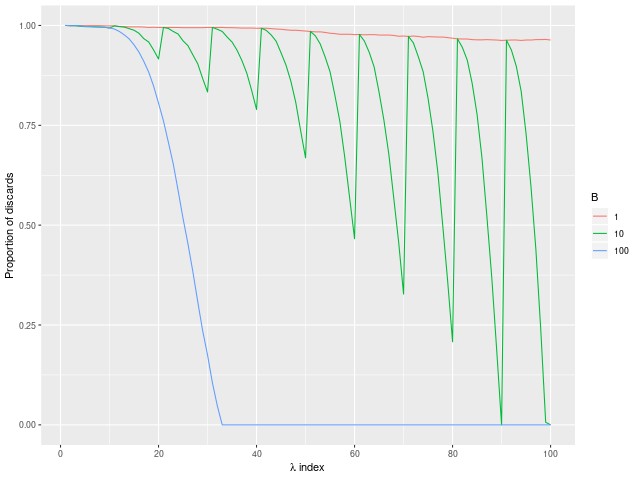
\includegraphics[scale = 0.5]{plots/batchsizes.png}    \caption{Proportion of features rejected by screening rules vs index of $\lambda$-values for different update delay.}
    \label{fig:3.4.1}
\end{figure}

BEDPP (Basic EDPP) rule is the special case of adaptive EDPP that never updates ($B=K$). When the reference does not get updated for a long time, the safe rule screening will eventually fail to discard any features and make the KKT condition checking cost increase to its maximum $np$. SEDPP rule is the special case that updates at every $\lambda$ value ($B=1$). It remains very powerful along the path, making the KKT condition checking cost small, but the safe screening itself is costly and takes $np$ time per $\lambda$-value. Adaptive EDPP can strike a balance between BEDPP and SEDPP. In this example, simply using fixed update period $B=10$ can reduce the safe screening cost by 90\% compared to SEDPP and reduce the KKT checking cost by 50\% to more than 90\% compared BEDPP.

This example also shows the timing of updates should be decided carefully and adaptively. For the first 10 $\lambda$-values, the safe rule stays powerful, which means the old reference is still exploitable. We may want delay the update to reduce average safe screening cost without harming the KKT condition checking cost much. For the last 20 $\lambda$-values however, the screening power drops to 0 quickly, which means the reference becomes useless quickly. Updating more frequently can greatly reduce the KKT condition checking cost with relatively small increase in safe screening cost. Also, the performance of adaptive EDPP rule also depends on many factors such as the data, the range of $\lambda$-values and spacing between $\lambda$-values. These suggest that simple updating rules like periodic updating cannot not be consistently efficient and we want a method that can automatically determine whether to update given current performance.

\subsubsection{Efficient updating algorithm}

From previous example, we assume the average cost is a convex function of distance from last update $B$, which decreases first and then after some optimal value increases again. If we want to minimize the average cost per $\lambda$-value, we need to update when using the old reference for one more $\lambda$-value will increase the average cost. That is, we should update the reference to $\lambda_{k+B}$ when $\bar{T}_k(B+1)>\bar{T}_k(B)$. For practice, we will update the reference to $\lambda_{k+B}$ when $\bar{T}_k(B)>\bar{T}_k(B-1)$ instead, because $\bar{T}_k(B+1)$ cannot be calculated without doing screening at $\lambda_{k+B+1}$. These two conditions should be close and thus this substitution should also be close to optimal. From (13), the latter condition will be:

\begin{equation}
    (B-1)|\mathcal{S}_{k+B}|-\sum_{b=1}^{B-1}|\mathcal{S}_{k+b}|>p.
\end{equation}


This updating condition is a greedy condition that only considers the cost up to the current $\lambda$ value. In practice, we cannot know about future $\lambda$ values so this is the most reasonable condition. In fact, it provides a robust strategy towards three most common scenarios. First, if the screening power stays high, meaning $\mathcal{S}_{k+b}$ is small for all $b$, then the left-hand-side of (14) will be small and thus at this point we will not update to further exploit the last update. Second, if the screening power has been high for a while but dropped suddenly, meaning $\mathcal{S}_{k+B}$ is large but $\mathcal{S}_{k+b}$ are mostly small for $b=1,2,...,B-1$, then the left-hand-side of (14) will be large and we will update the useless old reference to a new helpful one. Last, if the screening power drops dramatically right after the last update, meaning $\mathcal{S}_{k+b}$ are close to $p$ for $b=2,3,...,B$, then the left-hand-side of (14) will be approximately $p-|\mathcal{S}_1|<p$. We will not update although old reference is useless, because if we did, the new update would become useless quickly as well.

This adaptive updating condition fills in the condition on line 11 in Algorithm 2 and forms a complete pathwise lasso algorithm with adaptive safe strong screening. 


\section{Extension to other lasso type problems}
\label{sec:4}

The structure of the adaptive safe strong rule is easily extendable to any lasso problems that have corresponding sequential strong rule and sequential safe rule. After an adaptive safe strong rule is built, we can automatically apply the adaptive update algorithm to form a pathwise algorithm with adaptive safe strong screening. We are going to derive the extensions to two lasso type problems and show these extensions improve computation efficiency.

\subsection{Adaptive safe strong rule for sparse logistic regression}

The sparse logistic regression model can be defined as:

\begin{equation}
    \hat{\beta}(\lambda)=\underset{(\beta,\beta_0)\in \mathbb{R}^p\times\mathbb{R}^1}{\mathrm{argmin}}-\frac{1}{n}\sum_{i=1}^n\{y_i\log\pi_i(\beta)+(1-y_i)\log(1-\pi_i(\beta))\}+\lambda||\beta||_1,
\end{equation}
where $\pi(\beta)=\{\pi_i(\beta)\}_{i=1}^n=\{p(y_i=1|x_{i1},x_{i2},...,x_{ip})\}_{i=1}^n=\{e^{\eta_i(\beta)}/(1+e^{\eta_i(\beta)})\}_{i=1}^n$ is the predicted value vector and $\eta(\beta)=X\beta$ is the linear function. $X$ are still the $n\times p$ standardized feature matrix but in this model the $y\in\{0,1\}^n$ is an unstandardized binary response vector. $\beta$ is still the $p\times1$ coefficient vector but we also need a $\beta_0$ as the intercept.

We can use SSR to do the strong rule screening with a small change according to the KKT condition. The residual vector now is $r(\lambda_k)=y-\pi(\hat{\beta}(\lambda_k))$. Then the SSR discards the $j$-th feature at $\lambda_{k+1}$ if (4) holds.

For safe rule screening, instead of EDPP rules, Slores (sparse logistic regression screening rule)\citep{wang2014safe} is used. It was proposed as a one-step rule but it can be extended as a sequential rule with some minimal change and thus can be extended as adaptive rule. Let $\Tilde{y}=2y-1\in\{-1,1\}^n$, $r(\lambda_k)=y-\pi(\hat{\beta}(\lambda_k))$.

\begin{theorem}[Adaptive Slores]
For the sparse logistic regression model (15), let $\lambda_0:=\max_j|x_j^Ty/n|$, $\Tilde{y}=2y-1\in\{-1,1\}^n$. Suppose we have a sequence of $\lambda$ values $\lambda_0>\lambda_1>...>\lambda_K$. $\forall\theta\in(0,1)^n$, let 

\begin{equation}
    \begin{split}
        g(\theta)&=\frac{1}{n}\sum_{i=1}^n\{\theta_i\log \theta_i+(1-\theta_i)\log(1-\theta_i)\},\\
    \nabla g_i(\theta) &= \frac{1}{n}\log\frac{\theta_i}{1-\theta_i}.
    \end{split}
\end{equation}

Under condition (2) except for standardization for $y$, for any $k=1,2,...,K-1$, assume $\hat{\beta}(\lambda_k)$, $r(\lambda_k)=y-\pi(\hat{\beta}(\lambda_k))$, $x_*\in\{x_j:\hat{\beta}_j(\lambda_k)\neq0\} $, $\theta(\lambda_k)=\{r_i(\lambda_k)\Tilde{y}_i\}_{i=1}^n$ and $\hat{y}(\lambda_k):=\pi(\hat{\beta}(\lambda_k))$ are known. For any $k+b>k$, let

\begin{equation}
    R(\lambda_{k+b})=\sqrt{\frac{n}{2}\bigg[g\bigg(\frac{\lambda_{k+b}}{\lambda_k}\theta(\lambda_k)\bigg)-g\bigg(\theta(\lambda_k)\bigg)+\bigg(1-\frac{\lambda_{k+b}}{\lambda_k}\bigg)\bigg(\nabla g\big(\theta(\lambda_k)\big)\bigg)^T\theta(\lambda_k)\bigg]},
\end{equation}

$d(\lambda_{k+b})=\sqrt{n}(\lambda_k-\lambda_{k+b})/R(\lambda_{k+b})$. For $\xi = -1,1$ and $j=1,2,...,p$,

\begin{enumerate}
    \item If $-\xi sign(x_*^Ty)x_j^Tx_*\geq nd(\lambda_{k+b})$, then
    
    \begin{equation}
        T_\xi(\lambda_{k+b},x_j;r(\lambda_k))=\sqrt{n}R(\lambda_{k+b})-\xi x_j^Tr(\lambda_k);
    \end{equation}
    
    \item If $-\xi sign(x_*^Ty)x_j^Tx_*< nd(\lambda_{k+b})$, then
    
    \begin{equation}
        T_\xi(\lambda_{k+b},x_j;r(\lambda_k))=R(\lambda_{k+b})\sqrt{n+nu_\xi^2-2\xi u_\xi sign(x_*^Ty)x_j^Tx_*}-nu_\xi(\lambda_k-\lambda_{k+b})-\xi x_j^Tr(\lambda_k),
    \end{equation}
    where
    \begin{align}
        u_\xi&=\frac{-\xi a_1+\sqrt{\Delta}}{2a_2},\\
        a_0&=(x_j^Tx_*)^2-n^2d^2(\lambda_{k+b}),\nonumber\\
        a_1&=-2n\,sign(x_*^Ty)x_j^Tx_*\big(1-d^2(\lambda_{k+b})\big),\nonumber\\
        a_2&=n^2\big(1-d^2(\lambda_{k+b})\big),\nonumber\\
        \Delta&=a_1^2-4a_0a_1.\nonumber
    \end{align}
\end{enumerate}

Then $\hat{\beta}_j(\lambda_{k+b})=0$ if
        \begin{equation}
            \max_{\xi=\pm1} T_\xi(\lambda_{k+b},x_j;r(\lambda_k))
        \end{equation}
\end{theorem}

When computing the adaptive Slores, $\{x_j^Ty\}_{j=1}^p$ needs to be computed only once, stored and reused for the whole solution path. $\{x_j^Tx_*\}_{j=1}^p$ can be reused unless $x_*$ changes. Other than those two terms, the only term that requires expensive $O(np)$ computation is $\{x_j^Tr(\lambda_k)\}_{j=1}^p$, which only needs to be computed at the time of each update. Thus algorithm 2 for adaptive safe strong rule can be done with Slores rule instead of EDPP rule to form Ada-SSR-Slores that does screening for sparse logistic regression model.

\subsection{Adaptive safe strong rule for group lasso}

The group lasso problem \citep{yuan2006model} can be defined as:

\begin{equation}
    \hat{\beta}(\lambda) = \underset{\beta\in \mathbb{R}^p}{\mathrm{argmin}}\frac{1}{2n}\bigg|\bigg|y-\sum_{g=1}^GX_g\beta_g\bigg|\bigg|_2^2+\lambda\sum_{g=1}^G\sqrt{p_g}||\beta_g||_1,
\end{equation}
where $\beta=(\beta_1^T,...,\beta_G^T)^T$, $X_g$ is a $n\times p_g$ sub-matrix consisting of columns of $X$ corresponding to features in group $g$, $g=1,2,...,G$. Besides standardization in (2), we apply an addition level of standardization at the group level\citep{breheny2015group}:

\begin{equation}
    X_g^TX_g=nI_{p_g\times p_g},\qquad g=1,2,...,G.
\end{equation}

According to the KKT condition, we can use SSR to do strong rule screening. Given $r(\lambda_k)=y-\sum_{g=1}^GX_g\hat{\beta}_g(\lambda_k)$, we discard features in the $g$-th group at $\lambda_{k+1}$ if:

\begin{equation}
    \bigg|\bigg|\frac{1}{n}X_g^Tr(\lambda_k)\bigg|\bigg|_2<\sqrt{p_g}(2\lambda_{k+1}-\lambda_k).
\end{equation}

For safe rule screening, we have SEDPP for group lasso\citep{wang2013lasso} and we can extend it the adaptive EDPP rule for group lasso.

\begin{theorem}[Adaptive EDPP for group lasso]
For the group lasso problem (22), let $\lambda_0:=\max_j\frac{||X_g^Ty||_2}{n\sqrt{p_g}}$. Suppose we have a sequence of $\lambda$ values $\lambda_0>\lambda_1>...>\lambda_K$. Under condition (2) and (23)
    \begin{enumerate}
        \item For any $k=1,2,...,K-1$, given $\hat{\beta}(\lambda_k)$, $r(\lambda_k)$ and $\hat{y}(\lambda_k):=\sum_{g=1}^GX_g\hat{\beta}_g(\lambda_k)$, then for any  $k+b>k$, $\hat{\beta}_g(\lambda_{k+b})=0$ if
        \begin{equation}
            \begin{split}
                &\left|\left|2\lambda_{k+b}X_g^Tr(\lambda_k)+(\lambda_k-\lambda_{k+b})\left( X_g^Ty-\frac{y^T\hat{y}(\lambda_k)X_g^T\hat{y}(\lambda_k)}{||\hat{y}(\lambda_k)||_2^2}\right)\right|\right|_2\\
                &<2n\lambda_k\lambda_{k+b}\sqrt{p_g}-(\lambda_k-\lambda_{k+b})\sqrt{n||y||_2^2-\frac{n(y^T\hat{y}(\lambda_k))^2}{||\hat{y}(\lambda_k)||_2^2}}
            \end{split}
        \end{equation}
        \item For k=0, i.e., $\lambda_k=\lambda_0$, let $X_*=argmax_{X_g}\frac{||X_g^Ty||_2}{n\sqrt{p_g}}$ with dimension $n\times p_*$, then for any $b>0$, $\hat{\beta}_g(\lambda_{k+b})=0$ if
        \begin{equation}
        \left|\left|(\lambda_0+\lambda_b)X_g^Ty-(\lambda_0-\lambda_b)X_g^TX_*X_*^Ty\right|\right|_2<2n\lambda_0\lambda_b\sqrt{p_g}-(\lambda_0-\lambda_b)\sqrt{n||y||_2^2-n^2\lambda_0^2p_*}.
    \end{equation}
    \end{enumerate}
\end{theorem}

Similar to Adaptive EDPP rule, three expensive computations are $\{X_g^Ty\}_{g=1}^G$, $\{X_g^TX_*\}_{g=1}^G$ and $\{X_g^Tr(\lambda_k)\}_{g=1}^G$. The first and second only need to be computed once for the whole solution path. The last only needs to be computed at the time of each update with cost $O(np)$. The adaptive EDPP for group lasso, combined with the previous SSR, forms the Ada-SSR-EDPP for group lasso.

\section{Experiments}
\label{sec:5}

In this section conduct experiments solving lasso model on both simulated data sets and real data sets, to show our proposed adaptive safe strong rule screening method outperforms previous screening method such as SSR, SEDPP, HSSR and Slores. Active-set cycling in \ref{sec:active} is always used with all screening methods because it can be easily combined with any screening methods with no extra cost.

The adaptive safe strong rule screening is implemented in the \textbf{R} package \textbf{biglasso} and we will use this package for our experiment. Compared to traditional packages that solve lasso problem, such as \textbf{glmnet}, \textbf{biglasso} focuses on efficiently solving lasso problem with high-dimensional data sets that have a large number of features. First, it utilized the memory-mapping techniques that stores the data set on the disk and reads in only the part of the data necessary for model solving. Second, it applied screening rules to reduce both the computation cost and memory cost as we have discussed. These two features together help \textbf{biglasso} to outperform other packages. We will show that our new screening method will result in a new version of the package that shows significant improvement compared to previous version. 

For all the following experiments, we will solve the lasso model along a path of $100$ $\lambda$-values with the maximum $\lambda_0=\max_j|x_j^Ty/n|$ determined by the data, the minimum $\lambda_K=0.05\lambda_0$ and the rest $\lambda$-values equally spaced between on log scale.

\subsection{Simulation study}
\label{sec:sim}

\subsubsection{Lasso model}

In this part, we will solve the standard lasso problem (1) with different screening methods: Active-set Cycling (AC) alone, SSR, SEDPP, HSSR and adaptive safe strong rule (ASSR). The safe rule used in ASSR will be adaptive EDPP rule. Note that AC is always incorporated with all other screening rules, so using AC alone can be considered as a baseline for this comparison.

The data will be simulated from the model: $y=X\beta+0.1\epsilon$. $X$ and $\epsilon$ are sampled i.i.d from $N(0,1)$. $\beta$ will have $s$ randomly selected elements equally spaced between $[-\beta_{max},\beta_{max}]$ and the rest $p-s$ elements are zeros. Each setting is replicated $10$ times to calculate the average time cost. We consider the following cases:

\begin{enumerate}
    \item \textbf{Varying number of features $\mathbf{p}$:} we fix $n=1,000$, $s=20$, $\beta_{max}=1$ and vary $p$ from $1,000$ to $100,000$.
    \item \textbf{Varying sample size $\mathbf{n}$:} we fix $p=10,000$, $s=20$, $\beta_{max}=1$ and vary $n$ from $200$ to $10,000$.
    \item \textbf{Varying signal strength $\mathbf{\beta_{max}}$:} we fix $p=10,000$, $n=1,000$, $s=20$ and vary $\beta_{max}$ from $0.05$ to $1$.
    \item \textbf{Varying sparsity $\mathbf{s}$:} we fix $p=10,000$, $n=1,000$, total signal size $\beta_{max}\times s=20$ and vary $s$ from $10$ to $300$.
\end{enumerate}

\begin{figure}[h]
    \centering
    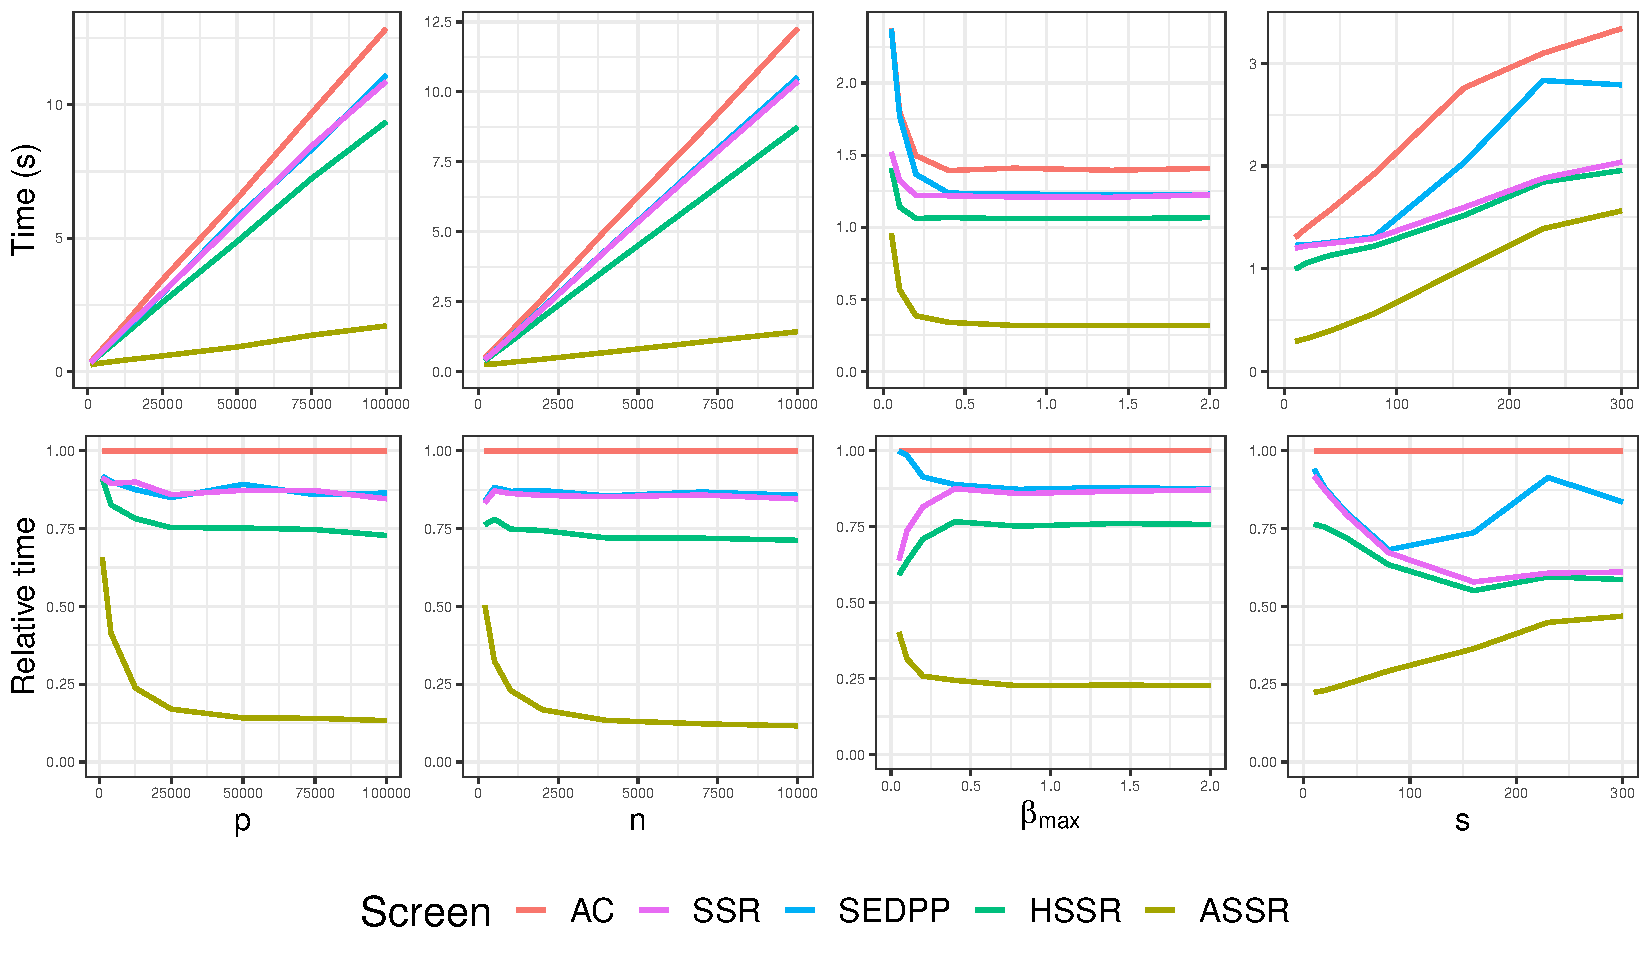
\includegraphics[scale = 0.59]{plots/gaus1.pdf}    \caption{Comparing speed of screening methods for lasso model under different settings. Top row: computation time in second. Bottom row: relative computation time compared to AC. First column: varying number of features $p$. Second column: varying sample size $n$. Third column: varying signal strength $\beta_{max}$. Fourth column: varying sparsity $s$.}
    \label{fig:5.1.1}
\end{figure}

Figure 2 shows the computation time (top row) and relative computation time compared to AC (bottom row) of solving lasso problem with different screening methods. The ASSR is uniformly the fastest under all settings. Most of the time it is 2-4 times faster than any other screening methods. It outperforms other methods especially when the data set is large (large $n$ or large $p$) or the active features are sparse among all features (small $s$). 

There are several atypical cases when ASSR's advantage over other methods is not as significant: (1) $p$ or $n$ is small. This corresponds a small data set and computation will be less challenging. (2) $\beta_{max}$ is close to zero. This means all the nonzero coefficients are close to zero and are hard to be distinguished from zero coefficients. This can cause problem for any statistical learning methods. (3) $s$ is large. In this case, the underlying model that generate the data set is not sparse in the sense that proportion of nonzero coefficients is not small. Lasso model would not be the optimal model to analyse such an data set.

We also tried varying other factors, for example, varying the correlation among features in $X$ or varying the sparsity with fixed signal strength. The ASSR also shows uniform advantage over other method when those factors vary in reasonable ranges.

\subsubsection{Sparse logistic regression model}

In this part, we will replicate the previous experiment, expect that now we will solve the sparse logistic regression model with the following screening methods: SSR, HSSR with Slores as the safe rule (HSlores), and ASSR with Slores as the safe rule (ASlores). SSR is implemented in all of the three screening methods so it will be considered as the baseline.

The data will be simulated from the model: $y=\mathbf{1}\{X\beta+0.1\epsilon >0\}$. $X$ and $\epsilon$ are sampled i.i.d from $N(0,1)$. $\beta$ will have $s$ randomly selected elements equally spaced between $[-\beta_{max},\beta_{max}]$ and the rest $p-s$ elements are zeros. Each setting is replicated $10$ times to calculate the average time cost. We consider the same 4 cases we have considered in the previous experiment.

\begin{figure}[H]
    \centering
    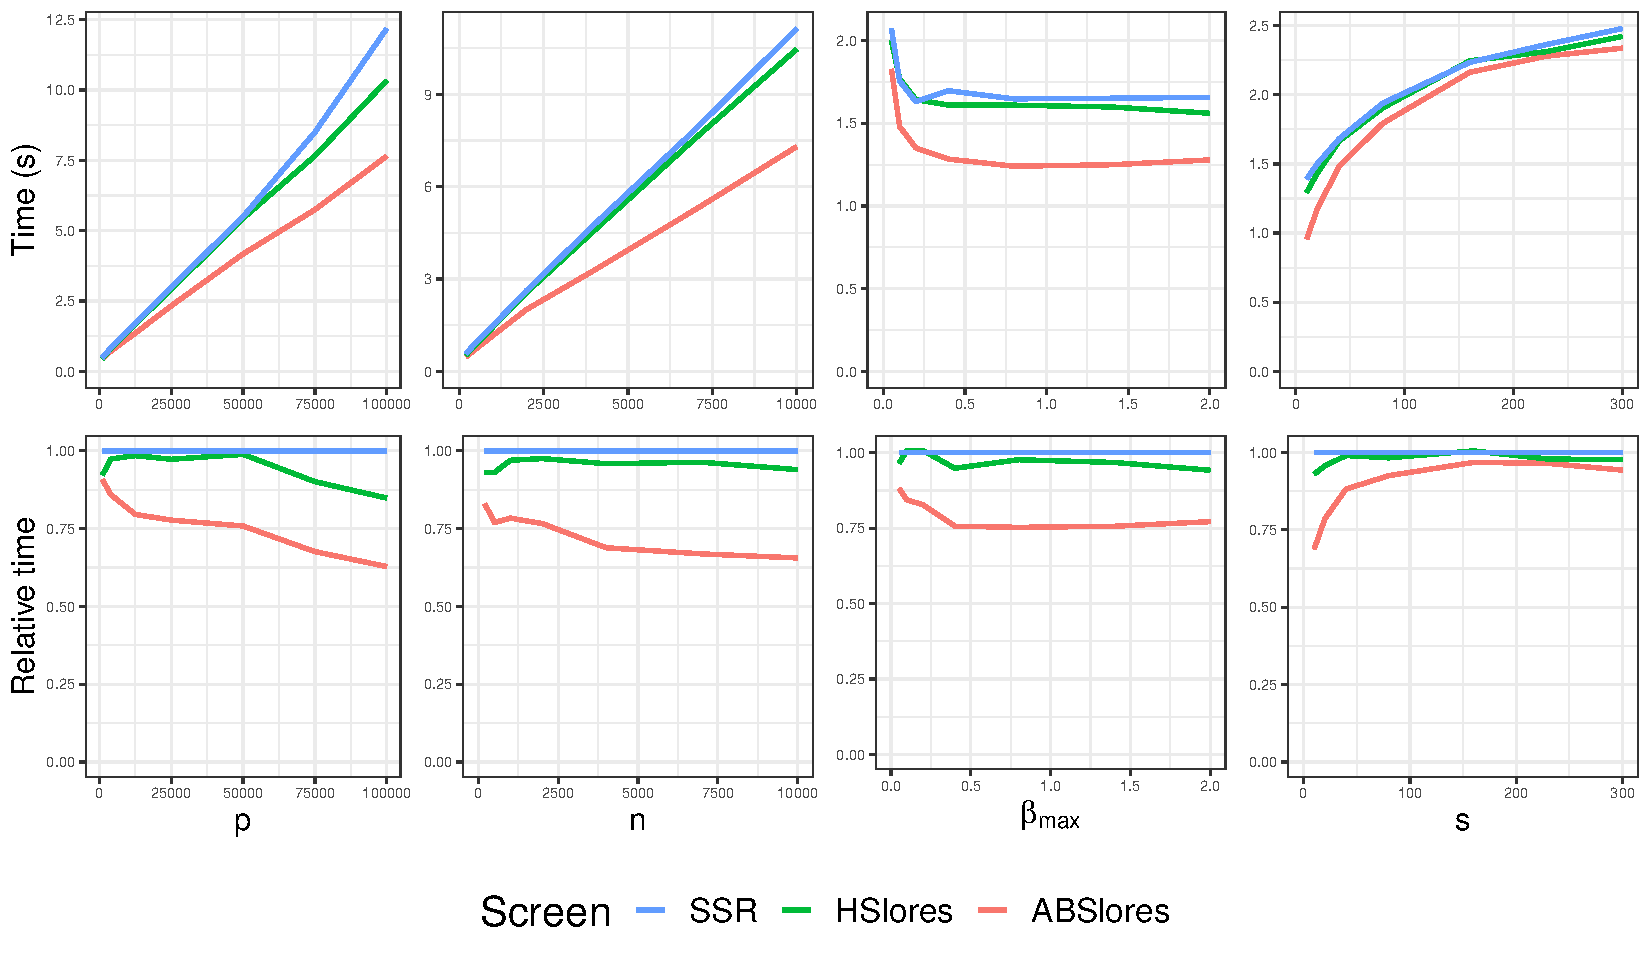
\includegraphics[scale = 0.59]{plots/bin1.pdf}    \caption{Comparing speed of screening methods for sparse logistic regression model under different settings. Top row: computation time in second. Bottom row: relative computation time compared to SSR. First column: varying number of features $p$. Second column: varying sample size $n$. Third column: varying signal strength $\beta_{max}$. Fourth column: varying sparsity $s$.}
    \label{fig:5.1.2}
\end{figure}

Figure 3 shows the computation time (top row) and relative computation time compared to SSR (bottom row) of solving sparse logistic regression problem with different screening methods. ASlores is also uniformly faster than other methods and this improvement is significant except for some atypical cases motioned before.


\subsection{Real data analysis}
\label{sec:real-data}

In previous sections, we used simulation to compare the screening methods under different scenario. In real world, data may be generated from different complicated models that cannot be covered by a simulation study, so in this section we are going to test these screening methods on some real data sets to make sure our comparison conclusion is representative in real world. Following the studies of \citep{wang2013lasso, xiang2016screening, zeng2017efficient}, we will test on the following data sets:

\begin{enumerate}
    \item \textbf{Breast cancer gene expression data
(GENE):} this data has expression measurements of $p=17,322$ genes from $n=536$ patients. The response is the expression measurement of the gene BRCA1, which has been identified to be related to risk of breast cancer.
    \item \textbf{MNIST handwritten image data
(MNIST):} this data set has $60,000$ images in the training set and $10,000$ images in the testing set. Each image is a $28\times 28=784$ pixels image of handwritten digits. We use the training set to form a $n=784\times p=60,000$ feature matrix, treating pixels as samples and images as features. Then an image from the testing set is randomly selected as the response.
    \item \textbf{ Cardiac fibrosis genome-wide association data
(GWAS):} this data set has $p=660,496$ single nucleotide
polymorphisms (SNPs) collected from $n=313$ human hearts. The response is the log of the ratio of cardiomyocytes to fibroblasts in the heart tissue, which is associated with heart failure.
    \item \textbf{Subset of New York Times bag-of-words data
(NYT):} the raw data set is a $300,000\times 102,660$ matrix, each row being a document and each column being number of occurrence of a specific word in those documents. We selected $n=5,500$ documents by removing documents with low word counts. Then $55,000$ words are selected as the features and a randomly selected word is the response.

\end{enumerate}


For 1 and 3, we replicate the experiment 10 times to take the average. For 2 and 4, since in each experiment the response is randomly selected, we replicate the experiment 50 times to get an accurate estimate. The following table compares the average computation time for different screening methods in these data sets.

\begin{table}[H]
\centering
\begin{tabular}{l|l|l|l|l}
\hline
 & GENE & MNIST & GWAS & NYT \\
Screening method & n=536 & n=784 & n=313 & n=5,500 \\
 & p=17,322 & p=60,000 & p=660,496 & p=55,000 \\ \hline
AC & 2.14 (0.03) & 6.82 (0.07) & 46.67 (0.13) & 59.20 (1.89) \\
SSR & 1.34 (0.01) & 5.20 (0.01) & 25.34 (0.08) & 35.40 (0.44) \\
SEDPP & 1.38 (0.01) & 8.40 (0.45) & 25.48 (0.05) & 53.69 (3.81) \\
HSSR & 1.21 (0.01) & 3.44 (0.07) & 23.85 (0.06) & 31.05 (0.80) \\
ASSR & \textbf{0.71 (0.01)} & \textbf{1.15 (0.02)} & \textbf{8.80 (0.03)} & \textbf{12.71 (1.05)} \\\hline
\end{tabular}
\caption{Average computing time in second (standard error) for solving the lasso model}
\end{table}

ASSR again outperforms other screening methods on all data sets, faster than the fastest of the rest by 70\% to 200\%. Also note that the performance of SEDPP varies a lot in MNIST and NYT data sets, where the response is randomly selected in each replication, suggesting that the speed of SEDPP is sensitive to the data. ASSR is built with SEDPP as the safe rule but does not have the problem of instability, because it can adaptively adjust itself according the performance of the safe rule.



\subsection{Big data performance}

\begin{itemize}
    \item Analyse and profile different methods. Compare them in big data case ?
\end{itemize}

\section{Conclusion}
\label{sec:6}

In this paper, we proposed the novel adaptive safe strong screening framework for efficient lasso type problem optimization over the solution path. The key idea is cleverly reusing the reference for screening along the path until updating to a new reference is beneficial for computation cost.  We developed three instances in this framework: Ada-SSR-EDPP, Ada-SSR-Slores and Ada-SSR EDPP for group lasso, for 3 different types of lasso problems. We tested the first two in extensive numeric experiments on both simulated data and real data, including a ultra big data that does not fit into the memory. Our proposed rules outperformed other state-of-the-art screening methods uniformly, especially in the most challenging scenarios. 

Ada-SSR-EDPP and Ada-SSR-Slores have been implemented in  publicly accessible \textbf{R} packages \textbf{biglasso}\citep{zeng2017biglasso}, which was used to carry out the numeric experiments.

Our adaptive safe strong screening framework also has great flexibility for extensions. It can substitute coordinate descent with any other faster lasso problem optimizer, SSR with any other stronger strong rules and the adaptive updating algorithm with any other cleverer algorithm. Most importantly, most sequential safe rules can be modified as adaptive safe rules and fit into our framework. This lead to several future extensions. First, if a stronger safe rule is developed, our framework can better exploit its power and lead to an even faster algorithm. Second, there are still many lasso type problems that do not have corresponding sequential safe rules, such as sparse Cox regression, sparse Poisson regression and sparse SVM. Once they are developed, they can be fit into our framework to produce efficient algorithm for other types of lasso problem.

\bibliography{ref}

\end{document}
